The Merlion water quality modeling framework is provided with WST to enable
fast multi-scenario simulations and solution of optimization problems that require
an embedded water quality model (e.g., booster placement with \code{booster\_mip}, source identification MIP formulation). 
In this section, the model equations and the calculations performed inside WST 
in order to generate a linear system of equations to describe the water
quality in a network are briefly described. The equations and the discretization process described in 
this section do not require any additional work from the user (except for selecting the merlion 
option in the configuration file). More details about the Merlion modeling framework is provided in \citep{Merlion12}.   
      
The model formulation ensures mass balances
at all junctions, pipes and tanks. The following mass balance equations
describe the transport of a species inside the network. For simplicity,
complete instantaneous mixing is assumed for the tanks, and plug flow
is assumed for the pipes.

\bigskip{}

\begin{equation}
c_{n}(t)=\dfrac{\sum_{i\in\Gamma_{n}^{O}(t)}Q_{i}(t)\hat{c}_{i}^{O}(t)-\sum_{i\in\Gamma_{n}^{I}(t)}Q_{i}(t)\hat{c}_{i}^{I}(t)+m_{n}(t)}{\sum_{i\in\Gamma_{n}^{O}(t)}Q_{i}(t)-\sum_{i\in\Gamma_{n}^{I}(t)}Q_{i}(t)+Q_{n}^{ext}(t)},\;\;\forall\;
n\in\mathbf{J} \label{eq:junctionbalance}
\end{equation}

\medskip{}

\begin{multline}
V_{n}(t)\dfrac{dc_{n}(t)}{dt}=\sum_{i\in\Gamma_{n}^{O}(t)}Q_{i}(t)\hat{c}_{i}^{O}(t)-\sum_{i\in\Gamma_{n}^{I}(t)}Q_{i}(t)\hat{c}_{i}^{I}(t)+m_{n}(t)\\
-\left[\sum_{i\in\Gamma_{n}^{O}(t)}Q_{i}(t)-\sum_{i\in\Gamma_{n}^{I}(t)}Q_{i}(t)+Q_{n}^{\mathrm{ext}}(t)\right]c_{n}(t),\;\;\forall\; n\in\mathbf{ST}\label{eq:tankbalance}
\end{multline}

\bigskip{}

\begin{equation}
\dfrac{\partial\hat{c}_{i}(x,t)}{dt}+u_{i}(t)\dfrac{\partial\hat{c}_{i}(x,t)}{dx}=0,\forall i\in\mathbf{P}\label{eq:pipebalance}
\end{equation}

where $c_{n}$ and $m_{n}$ denotes the concentration and mass injected at a node,
respectively. The variable $\hat{c}_{i}$ is the concentration inside pipe $i$ 
and $V_{n}$ is the volume of water inside tank $n$.
The variable $\mathbf{{J}}$ is a set of all junctions, $\mathbf{{ST}}$
is a set of all storage tanks and $\mathbf{{P}}$ is a set of all
pipes. The variable $Q$ denotes volumetric flow rates that are pre-calculated using
EPANET 2.00.12 and are assumed to be constant over each hydraulic time step.
The flow rate of a known external source entering a node is also pre-calculated
and is denoted by $Q_{i}^{\mathrm{ext}}$. The variable $\Gamma_{n}^{O}$ represents the
set of all pipes with flow going away from node $n$. Similarly,
$\Gamma_{n}^{I}$ represents the set of all pipes with flow coming
into node $n$. 

Equation~\ref{eq:junctionbalance} represents a set of algebraic equations
dependent on time alone and Equation~\ref{eq:tankbalance} represents
a set of ordinary differential equations (ODEs) also dependent on time alone. Therefore, these two equations
can be discretized in time. However, discretizing Equation~\ref{eq:pipebalance},
which are partial differential equations (PDEs), in both time and space would lead to a prohibitively
large model. Instead, these pipe balance PDEs are replaced using an origin-tracking
algorithm. This algorithm is based on the Lagrangian method; however,
instead of tracking concentration values as packets of water moving
through the network, the origin-tracking algorithm tracks the originating
node and time step of each packet as it enters a pipe (see Figure \ref{fig:origin_figure}). 
Once the water packet exits the pipe, equations are written relating
the concentration of the pipe inlet and outlet to the concentration
of connected nodes based on time delay. These time delay expressions
are formulated for each pipe independently. Therefore, the algorithm
scales favorably for a large water distribution system having a linear
computational cost as the size of the network increases. 

\begin{figure}[!h]
\begin{center}
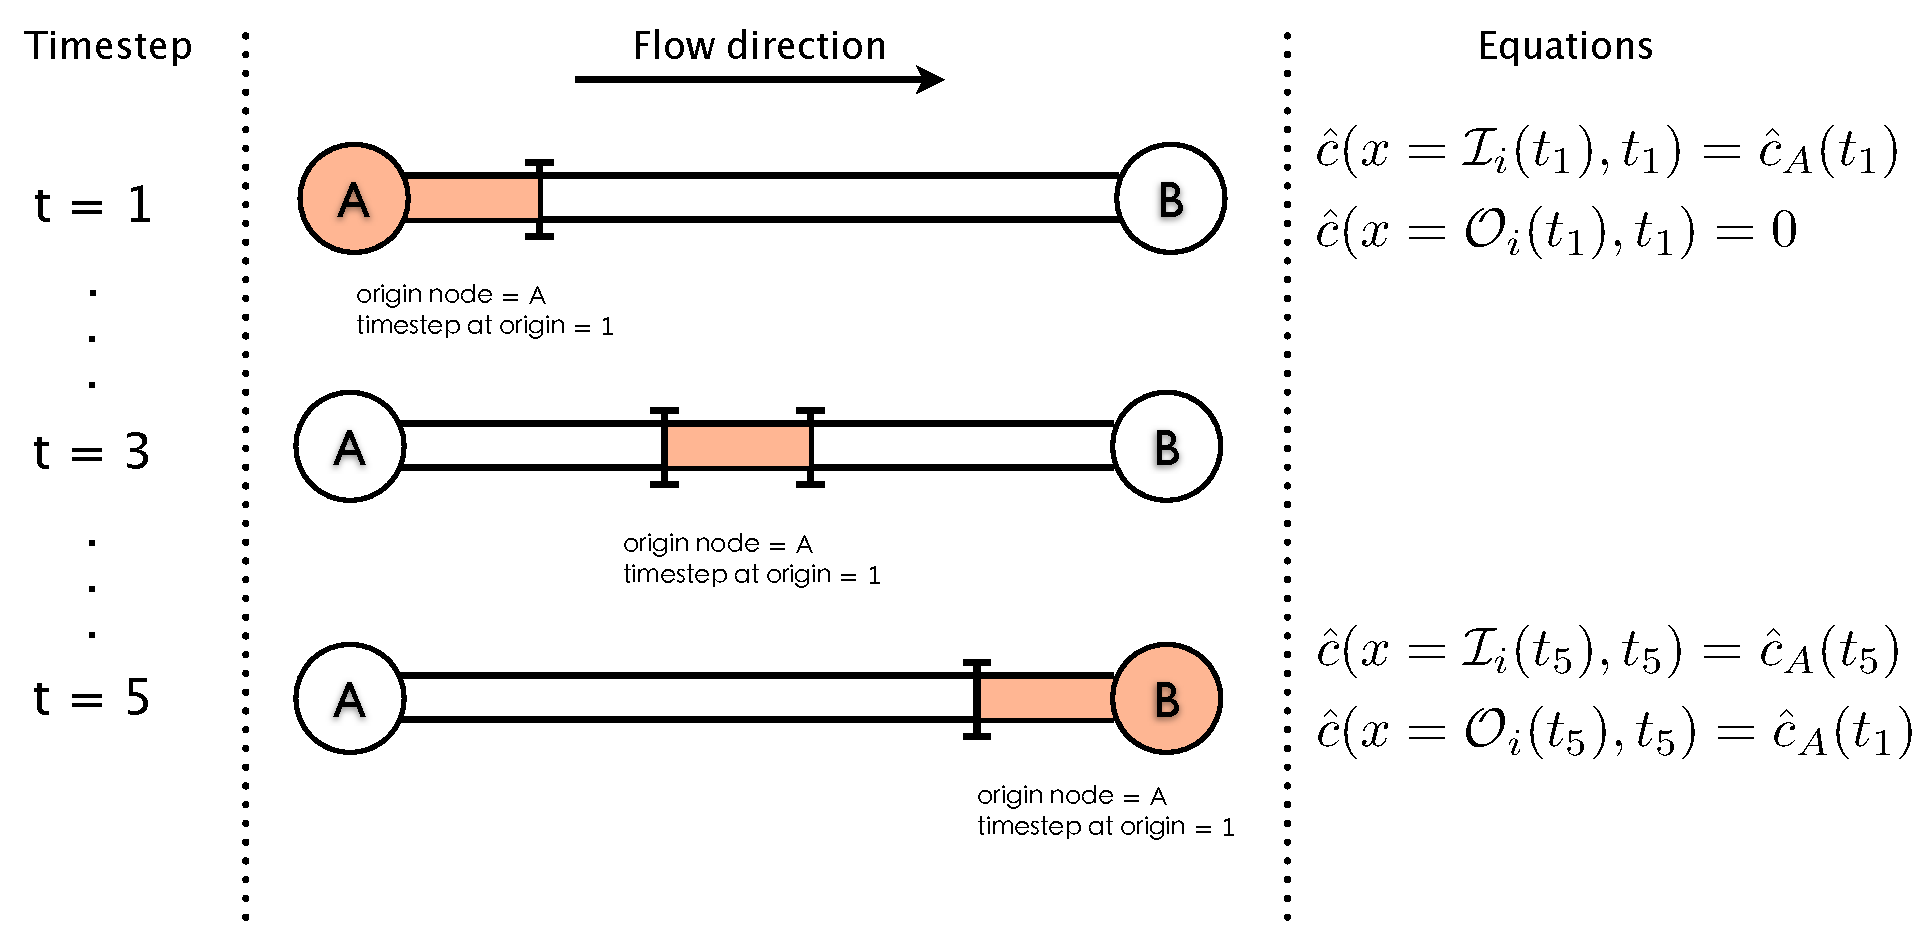
\includegraphics[scale=0.38]{graphics/origin_figure.pdf}\caption{Illustration of the origin tracking algorithm.}
\label{fig:origin_figure}
\end{center}
\end{figure}


By calculating time delay expressions, a very large but sparse linear
system of equations is generated that relates 
%The time delay expressions are included in the mass balance equations
%to form a large but very sparse linear system relating 
input injections ($m$)
from all nodes and time steps to output concentrations ($c$) from
all nodes and time steps.

\begin{equation}
Gc=Dm\label{eq:Merlion_Model}
\end{equation}


Unlike black box simulations, this linear model can be extended and
embedded inside other numerical applications. For example, the water quality model can be
embedded inside a mathematical programming formulation for applications
like booster placement, source inversion and optimal grab sampling. 

After formulating the linear system, performing a tracing simulation
is straightforward. First, an injection profile ($m$) is specified.
Then, the system is factorized and finally backsolved for the network
concentration profile $c$. This process is fast, and even more efficient
when simulating a large ensemble of tracing simulations. In this case,
the system is factorized once, and a backsolve is performed for each
simulation. To get additional speedup, a tailored solver is also provided
that takes advantage of the structure of the linear system by permuting
matrix $G$ into lower triangular, which removes the need for any
factorization. The tailored solver also utilizes the Basic Linear
Algebra Sub-routines (BLAS) library to perform multiple backsolves
(corresponding to multiple injection scenarios) more efficiently. 
For additional information about Merlion, refer to \citet{Merlion12}. 
%\mathbf{NOTE: Merlion currently only supports time based controls. 
%All EPANET networks INP files provided with WST have been modified by 
%converting all conditional controls to time based controls. This was 
%done by running the hydraulics and finding the first time at which a 
%conditional control was trigger and then enforcing a time based control 
%at the closest earlier hydraulic time step.} 
